\documentclass[12pt]{article}

\usepackage[english]{babel}
\usepackage[utf8x]{inputenc}
\usepackage{pdfpages}
\usepackage{lastpage} % Required to determine the last page for the footer
\usepackage{extramarks} % Required for headers and footers
\usepackage{graphicx} % Required to insert images
\usepackage{listings} % Required for insertion of code
\usepackage{courier} % Required for the courier font
\usepackage{color}
\usepackage{grffile}
\usepackage{float}

\usepackage[a4paper, total={6in, 8in}]{geometry}

% Margins
\topmargin=-0.45in
\evensidemargin=0in
\oddsidemargin=0in
\textwidth=6.5in
\textheight=9.0in
\headsep=0.25in
\fboxsep=0mm%padding thickness
\fboxrule=2pt%border thickness

\linespread{1.1} % Line spacing

\newcommand{\Title}{User manual} % Assignment title
\newcommand{\Class}{Cos\ 301} % Course/class
\newcommand{\pd}{Post-Doctoral}
\newcommand{\ssr}{Soft\color{green}{Serve }\color{black}}
\newcommand{\version}{1.0 (Final)}
\newcommand{\iteration}{6}
\newcommand{\client}{Ms. Cathy Sandis (UP DRIS)}
\newcommand{\supervisor}{Prof. Stefan Gruner (SSFM Group)}
\newcommand{\project}{Post-Doctoral management System}
\newcommand{\repo}{https://github.com/mox1990/Project-Postdoc.git}

\begin{document}


\vspace{4em}

\begin{center}%

\begin{figure}[ht!]
\centering

\includegraphics{../Images_Docs/logo.png}
\end{figure}
\LARGE \bf \Class \\[0.25em]
\LARGE \bf \project \\[1em]
\LARGE \bf \Title \\[0.25em]
\large \bf \today\\
\bf Version \version\\
\bf Iteration \iteration\\[0.5em]
\Large \bf Prepared for \\Client: \client\\Supervisor: \supervisor
\Large \\\bf by \\
\Large {\bf \ssr Group }\\[0.5em]
\LARGE {\bf Group members}\\[0.25em]
\large
Kgothatso Phatedi Alfred Ngako (12236731) \\[0.5em]
Tokologo “Carlo” Machaba (12078027) \\[0.5em]
Mathys Ellis (12019837) \\[8em]

\end{center}%

%\newpage
%{\LARGE \bf Change log}\\[2em]

\begin{center}
\begin{tabular}{|l|p{1.4cm}|p{8cm}|p{2.8cm}|}
\hline
\multicolumn{4}{|c|}{\bf Change log} \\
\hline
 Date & Version & Description &  Person \\
\hline
%10/02/2014 & v 0.0 & Document created & Mathys Ellis \\
%\hline
%02/03/2014 & v 0.1 & Added to glossary & Mathys Ellis \\
%\hline


%\end{tabbing}
\end{tabular}
\end{center}
\newpage
\tableofcontents

\listoffigures
\newpage

\section{Introduction}
Thank you for using the Post Doctoral Management System. The product is being developed using the process of software engineering according the IEEE standards and will be released as version 1 in the coming months.

The  current version is being released to get user input from the stakeholders so that improvements can be made to the product.

\section{What is a Post Doctoral Management System?}
The Post Doctoral Management System makes the management of the prospective and renewal application processes of Post-Doctoral fellowships, from start to end, more effective, intractable, reliable, secure and audit-able. And also provide the necessary auxiliary services to support the application process and make use of its data. The system makes use of a centralised user friendly web interface that will be used by the all the stakeholders involved in the various processes. The system hosts various sections that handle the different stages in the work-flow of the processes. The system automates the transitions between stages by forwarding the required information to the next stakeholder in the process and notifying them via an email notification or equivalent. The system will also need to provide reporting facilities for the application and person information stored by the system. As well as progress tracking with regards to any application. The system data is centralised to ensure that any information used by system is cohesive and valid for any stakeholder who accesses it. The system also allows for the recreation of existing data with regards to applications, people and locations, which act as importing facilities.

\section{Post Doctoral Management System for End Users}
The system is designed in such a way that it is accessible over any device that has access to the Internet via a web browser, whether over a computer, tablet or mobile phone. Once the user has accessed the system, it is simple for non-technical users to figure out how to navigate through the web application.

The system has a number of functions which are available to the end users depending on their security roles. Here is a list of all the functionality included in the system currently:
\begin{itemize}
\item Application Management Services
\item Notification Services
\item Announcements
\item User Account Management Services
\item Location Services
\item Meeting Management Services
\end{itemize}

and many more functions within the above mentioned functions.

\section{Objectives of the User Manaul}
The objectives of the User Manual are to:
\begin{itemize}
\item Provide instructions on how to access the system
\item Provide instructions on how to navigate through the system
\end{itemize}
This is not a Technical Manual in that we do not go in depth on the processes followed by each stakeholder and the various roles they perform through the process. It is expected that each stakeholder knows their role beforehand.

\newpage
\section{Getting Started}
The Post Doctoral Management System has been developed in a simple and understandable way. New users should not have any trouble using the system as it follows the standards that have been set in industry.

\section{System Requirements}
The system will run on the following web browsers and their mobile counterparts
\begin{enumerate}
\item Mozilla Firefox 20+
\item Google Chrome 30+
\item Microsoft Internet Explorer 9+
\item Apple Safari
\item Opera
\end{enumerate}

 \newpage
\section{Creating a User Account(Prospective Fellows)}
This process is a simple as a filling the form, once that is done an email will be sent to verify your details and to authenticate you are the user
\begin{figure}[H]
\centering	
\framebox{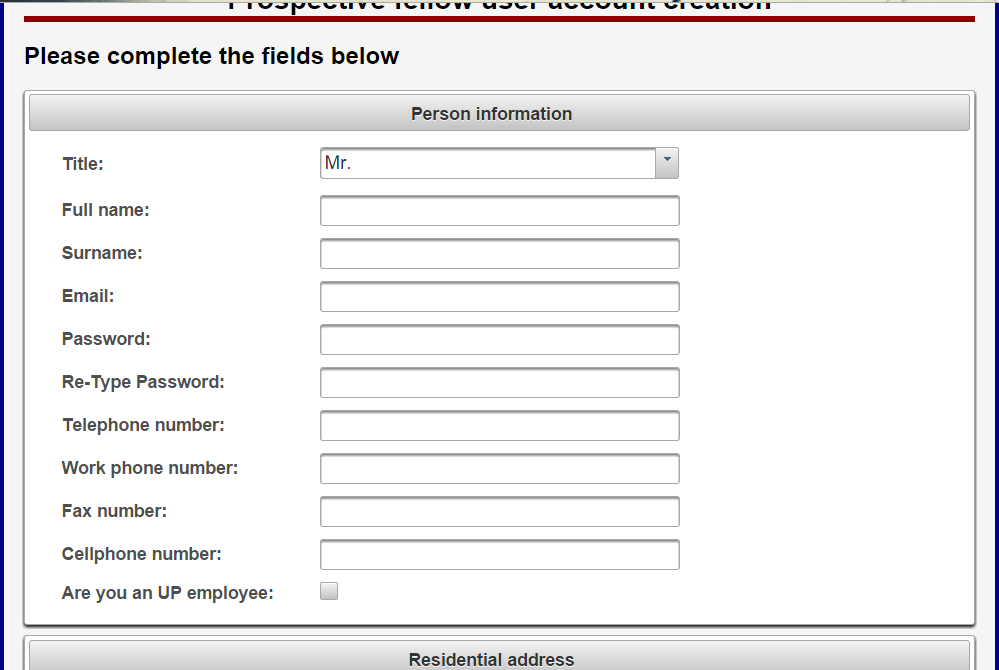
\includegraphics[scale=0.5]{../Images_Docs/Screenshots/CreateApp.png}}
\caption{Creating a User Account}
\end{figure}
 \newpage
 
\section{Logging on to the System}

Enter your user name and password
\begin{figure}[H]
\centering	
\framebox{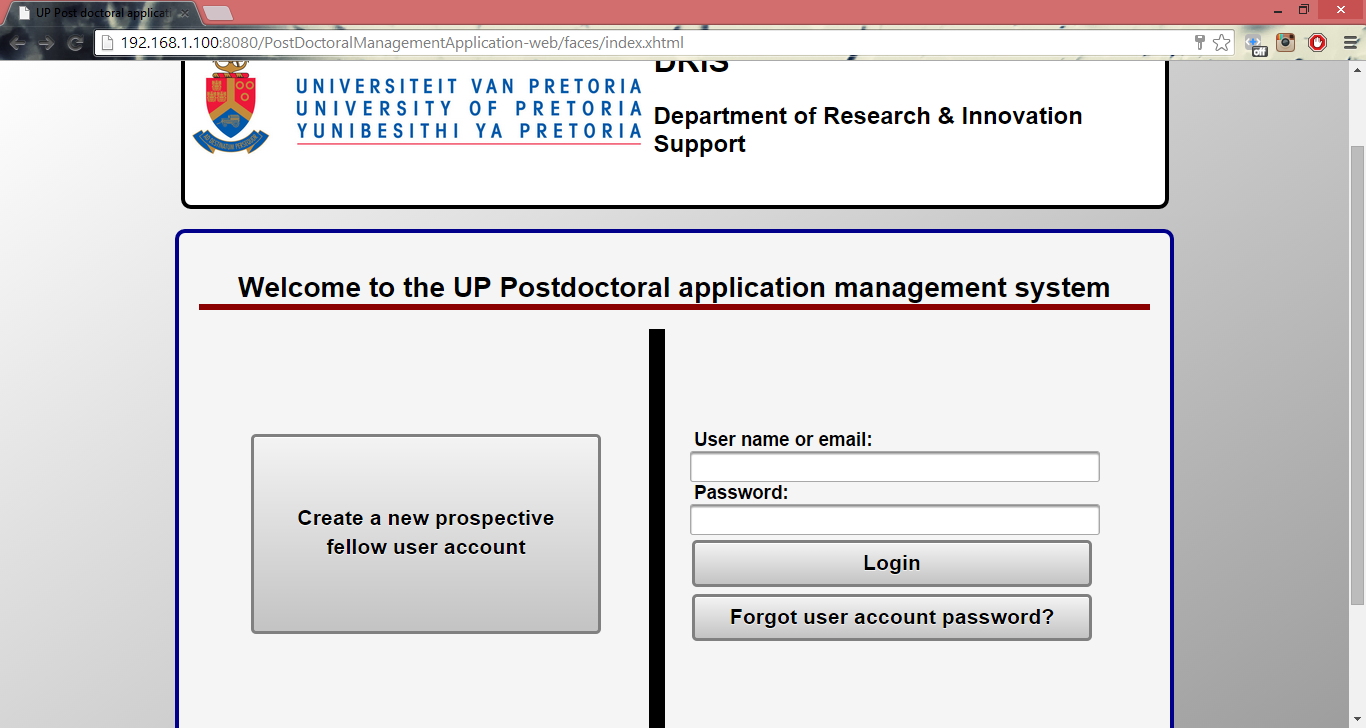
\includegraphics[scale=0.5]{../Images_Docs/Screenshots/homePage.png}}
\caption{Login}
\end{figure}

 \newpage
\section{Main Menu}
This is the main menu, depending on your security role you will see different items, double click to enter the service you want to use
\begin{figure}[H]
\centering	
\framebox{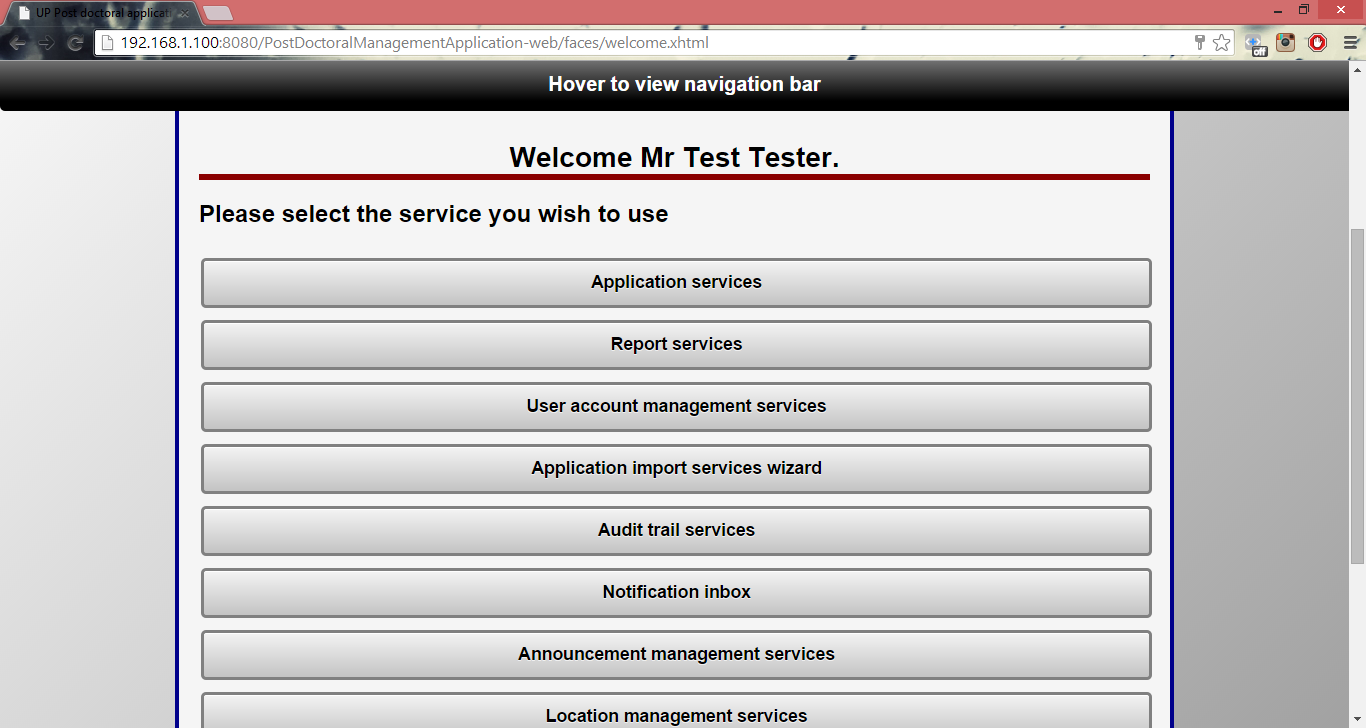
\includegraphics[scale=0.5]{../Images_Docs/Screenshots/menu.png}}
\caption{Main Menu}
\end{figure}

 \newpage
\section{Application Services}

This is the application service menu, depending on your security role you will see different items, double click to enter the service you want
\begin{figure}[H]
\centering	
\framebox{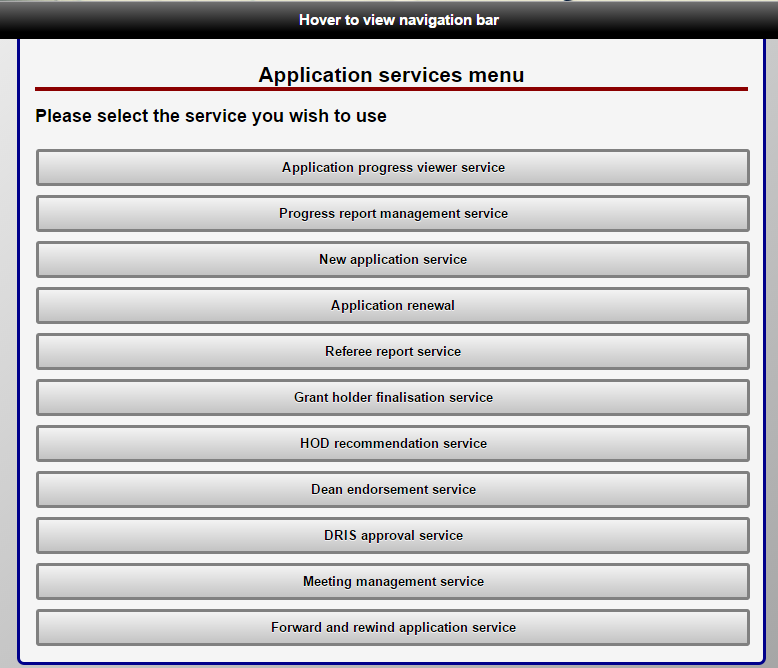
\includegraphics[scale=0.5]{../Images_Docs/Screenshots/AppServices.png}}
\caption{Application Services Menu}
\end{figure}

 \newpage

\section{Navigation Bar}
If you hover at the top of the page you will navigate through the system. It is availabe at the top of the page. If the user is not comfortable using this, the back button on the web browser works as well
\begin{figure}[H]
\centering	
\framebox{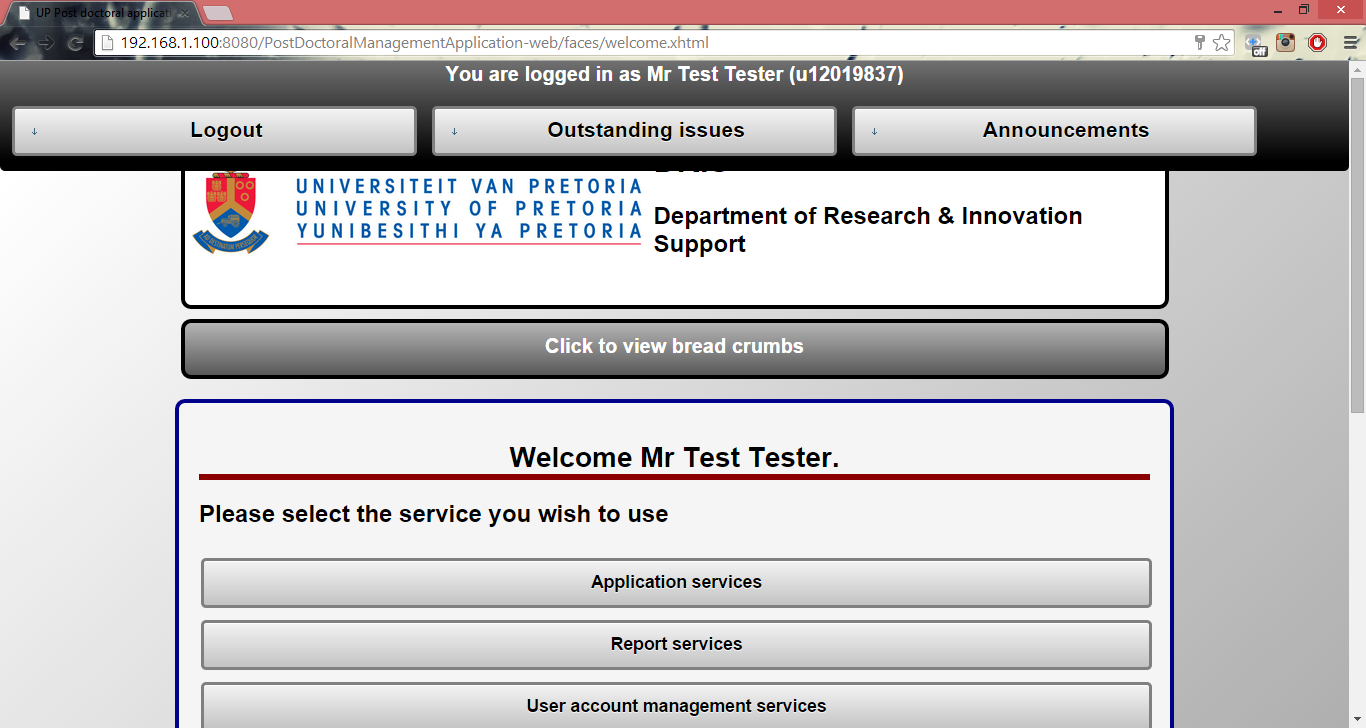
\includegraphics[scale=0.5]{../Images_Docs/Screenshots/navigationBar.png}}
\caption{Navigation Bar}
\end{figure}

 \newpage

\section{Bread Crumbs}
This shows the path followed to get to the state you are currently in, simply click on the button
\begin{figure}[H]
\centering	
\framebox{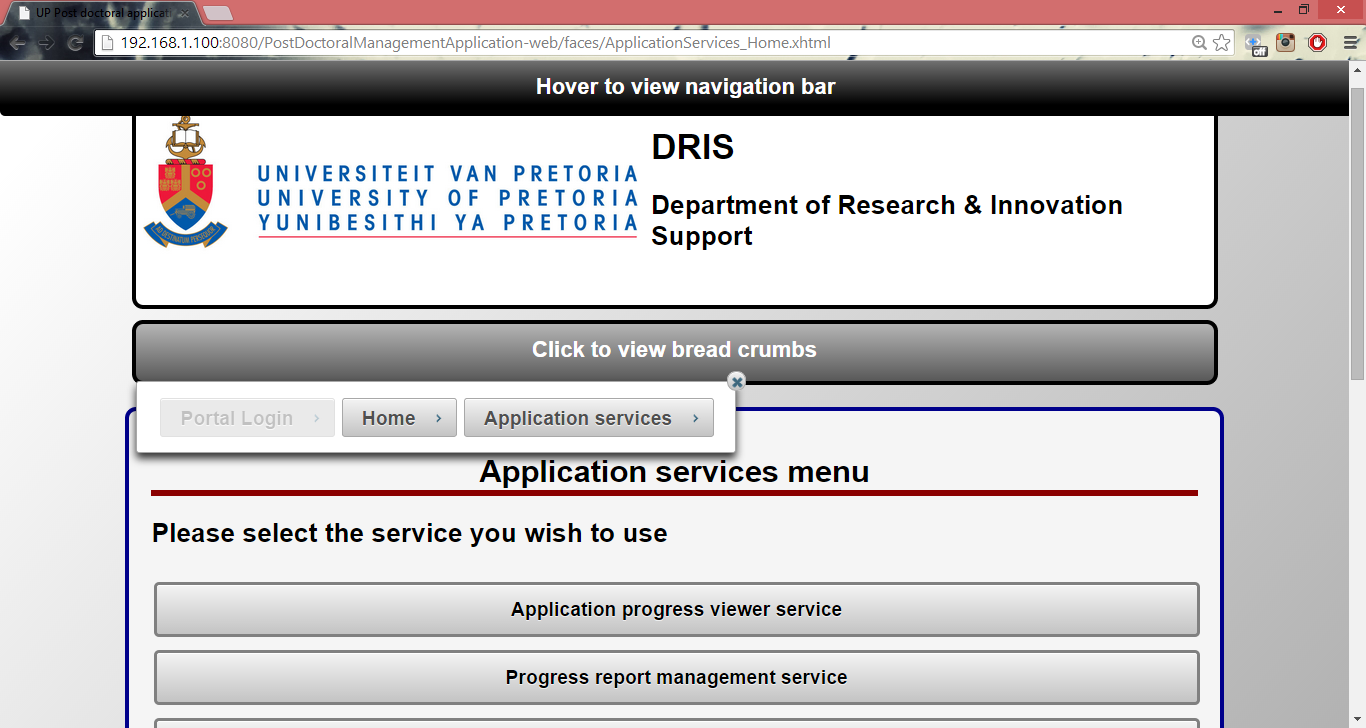
\includegraphics[scale=0.5]{../Images_Docs/Screenshots/BreadCrumbs.png}}
\caption{Bread Crumbs}
\end{figure}

\newpage
\section{Announcement Management}
The following provides the options available for users with regards to Announcement Management.

For announcement creation the user enters the details into the form and click on publish it once you are done.
\begin{figure}[H]
\centering	
\framebox{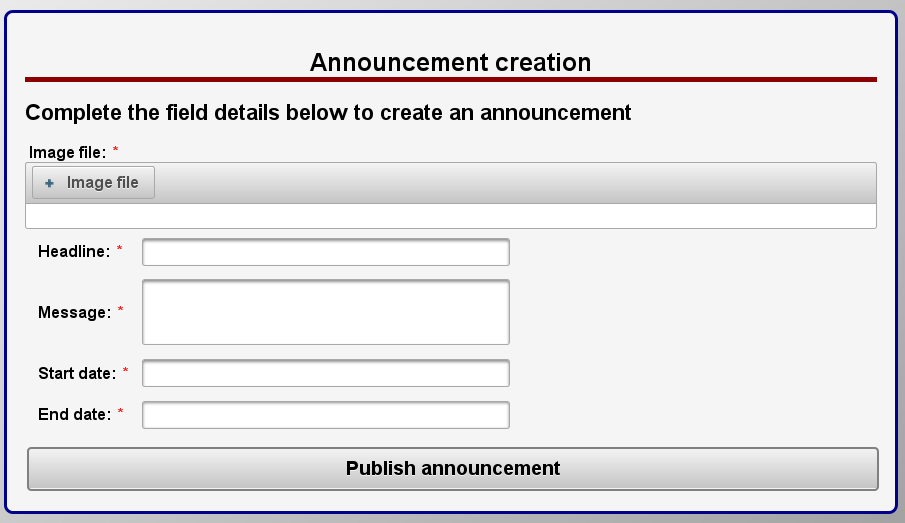
\includegraphics[scale=0.5]{../Images_Docs/Screenshots/AnnouncementManagementCreation.png}}
\caption{Creating an Announcement}
\end{figure}

\begin{figure}[H]
\centering	
\framebox{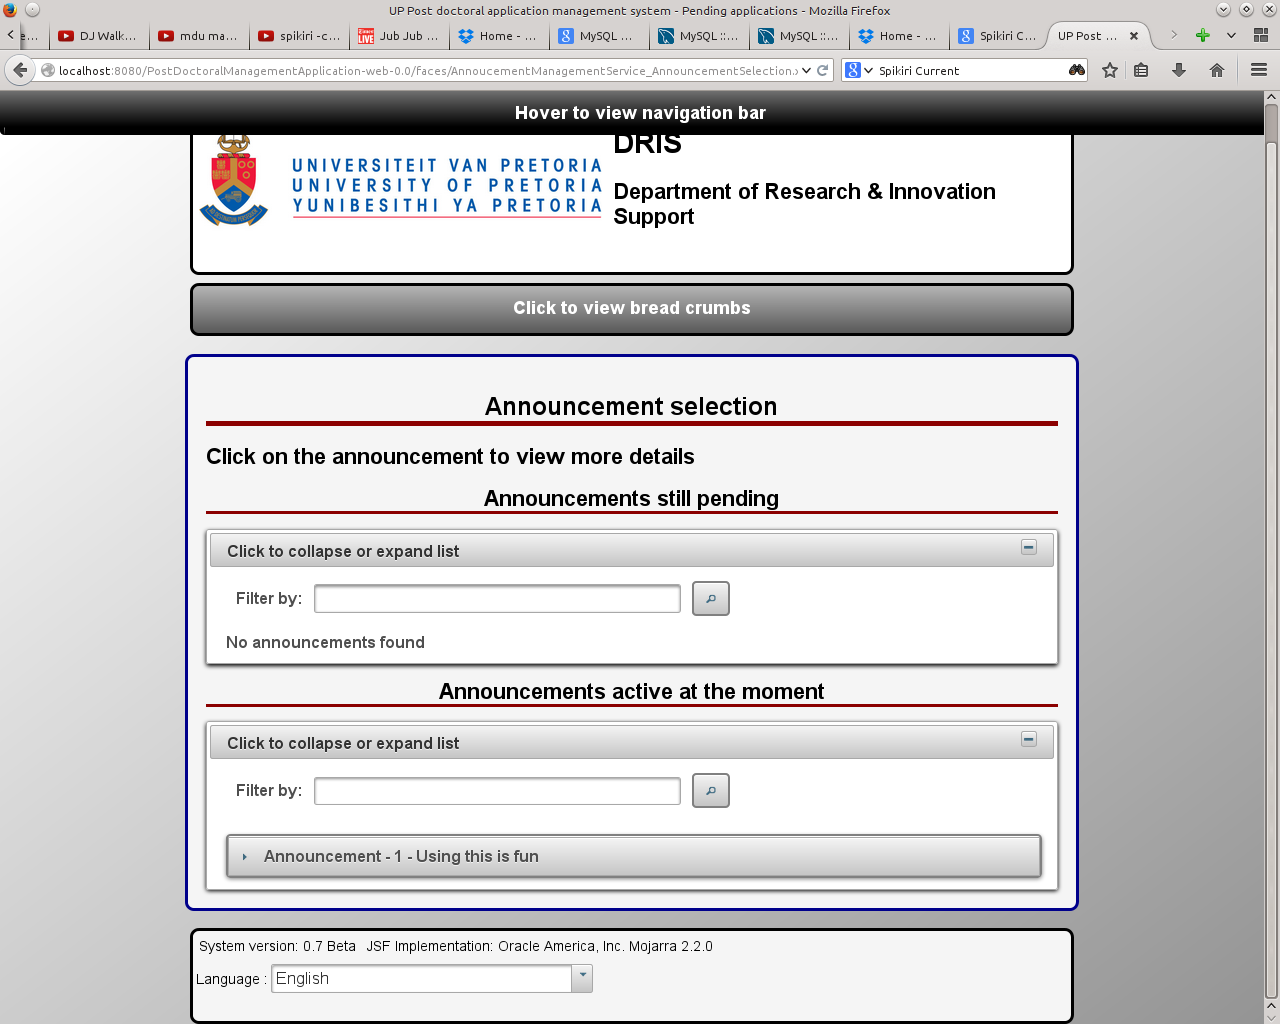
\includegraphics[scale=0.5]{../Images_Docs/Screenshots/AnnouncementManagementView.png}}
\caption{View all the Announcements}
\end{figure}

`\section{Audit Trail Services}
The user will be able to view the audit log, they can enter information in the filters to find the entries they would like to see
\begin{figure}[H]
\centering	
\framebox{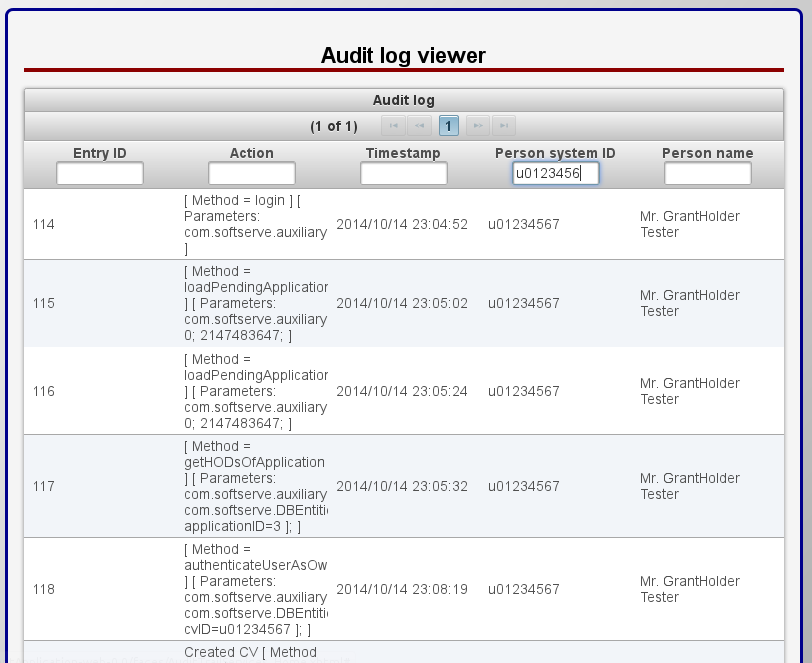
\includegraphics[scale=0.5]{../Images_Docs/Screenshots/AuditTrail1.png}}
\caption{View the audit log}
\end{figure}

\newpage
\section{Forward and Rewind Service}

The user will click on the application they wish to forward or rewind, change the application status and state the reason for the change
\begin{figure}[H]
\centering	
\framebox{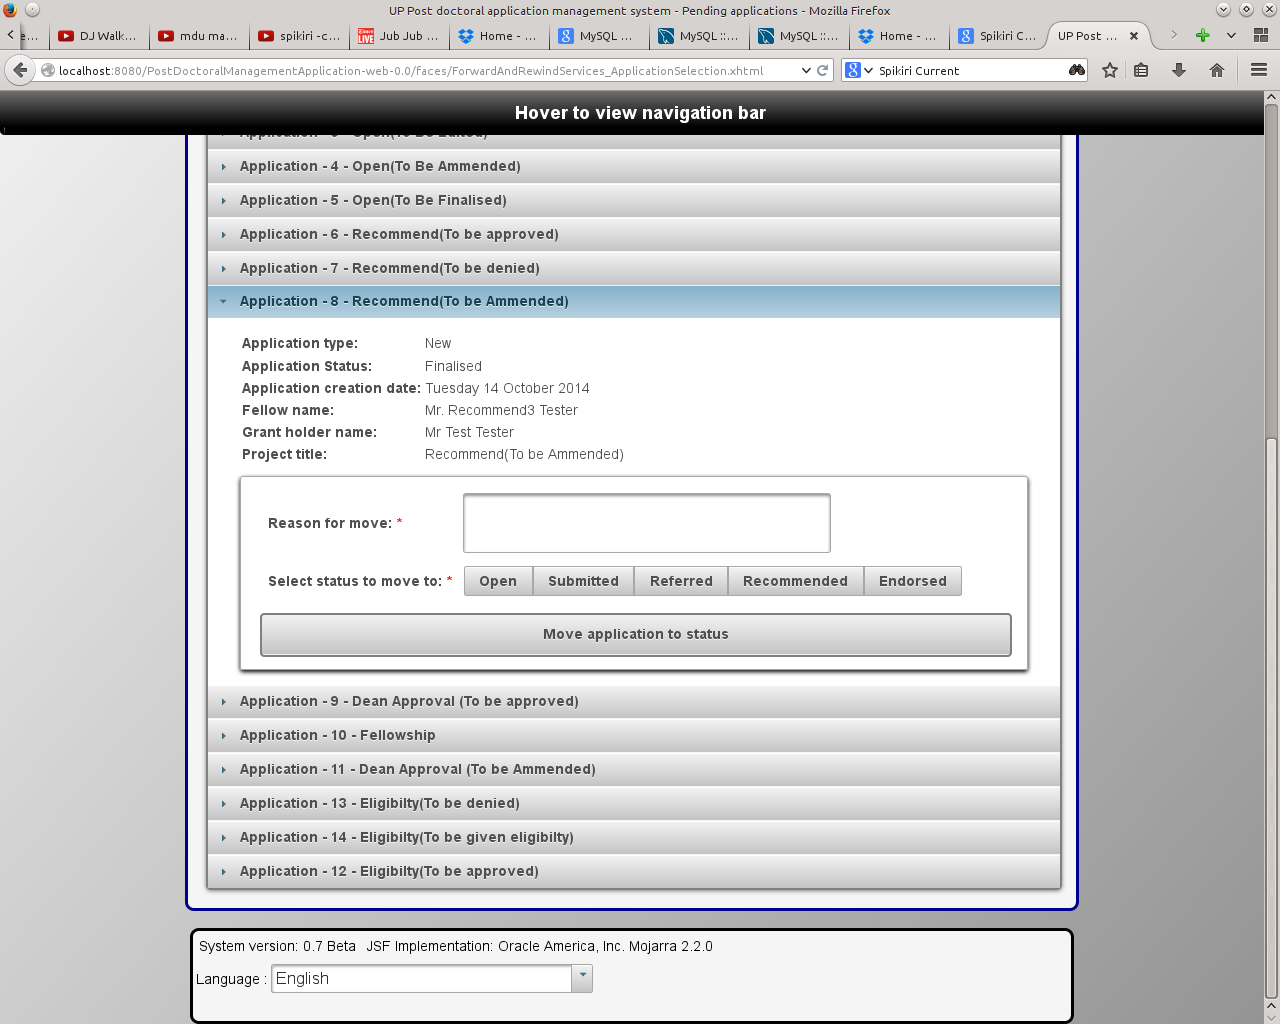
\includegraphics[scale=0.5]{../Images_Docs/Screenshots/FowardRewind1.png}}
\caption{Forward or Rewind An Application}
\end{figure}

\newpage
\section{Location Management Service}
The user will navigate through to the required location by double clicking on the appropriate button. At the bottom of the screen the user will be able to change the name of the location or create a new location.
\begin{figure}[H]
\centering	
\framebox{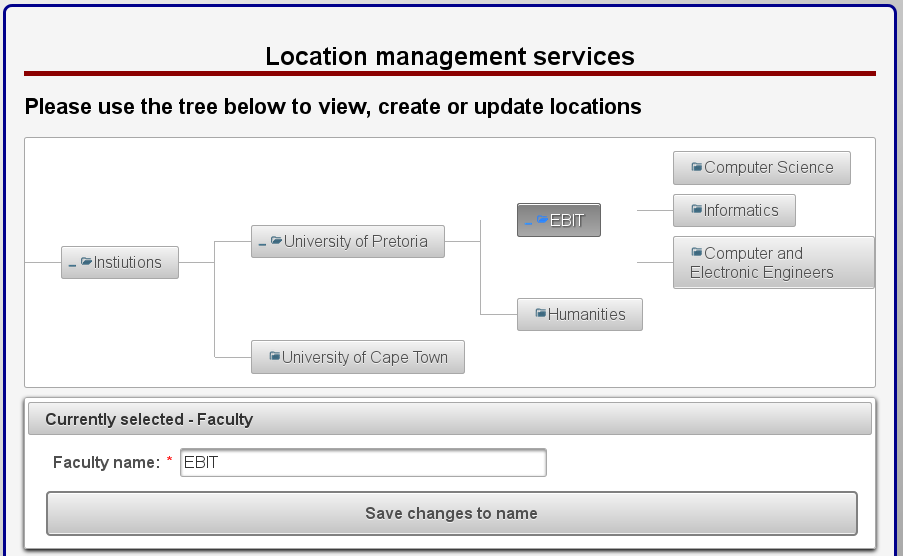
\includegraphics[scale=0.5]{../Images_Docs/Screenshots/LocationManagement3.png}}
\caption{Forward or Rewind An Application}

\end{figure}

\newpage
\section{Meeting Management}

\begin{figure}[H]
\centering	
\framebox{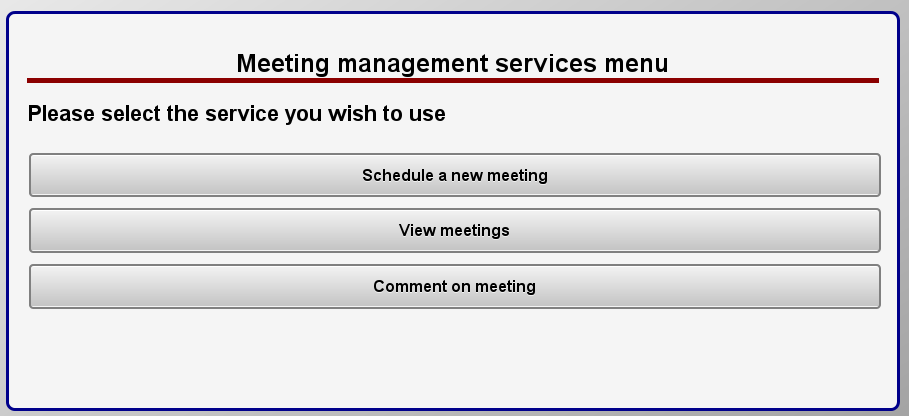
\includegraphics[scale=0.5]{../Images_Docs/Screenshots/MeetingManagement.png}}
\caption{Meeting Management Menu}
\end{figure}

The user will select the option they want from the menu above.
\begin{figure}[H]
\centering	
\framebox{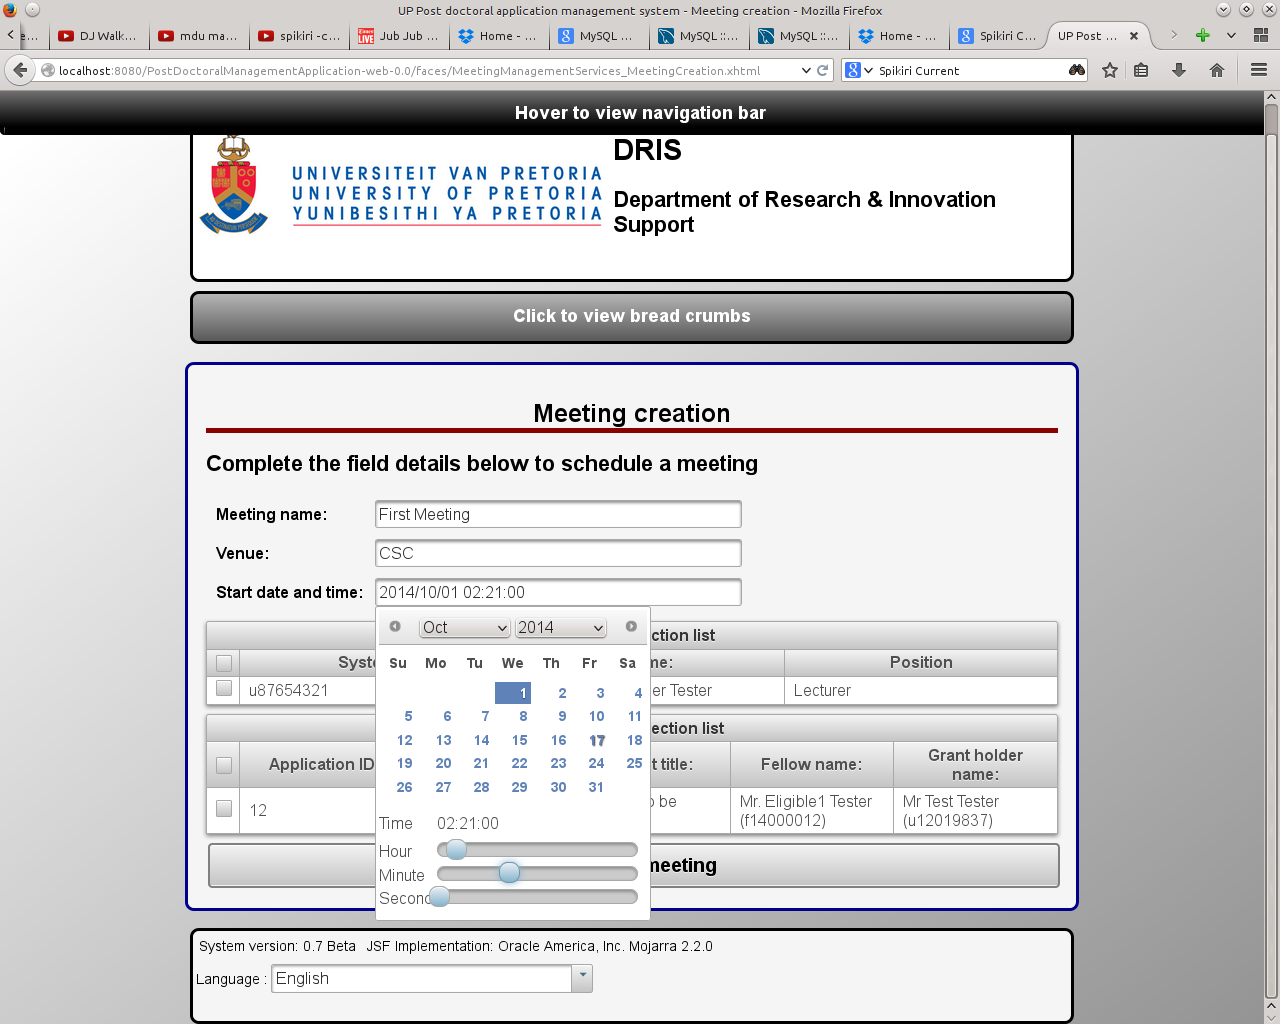
\includegraphics[scale=0.5]{../Images_Docs/Screenshots/MeetingManagementCreate1.png}}
\caption{Meeting Creation}
\end{figure}

\begin{figure}[H]
\centering	
\framebox{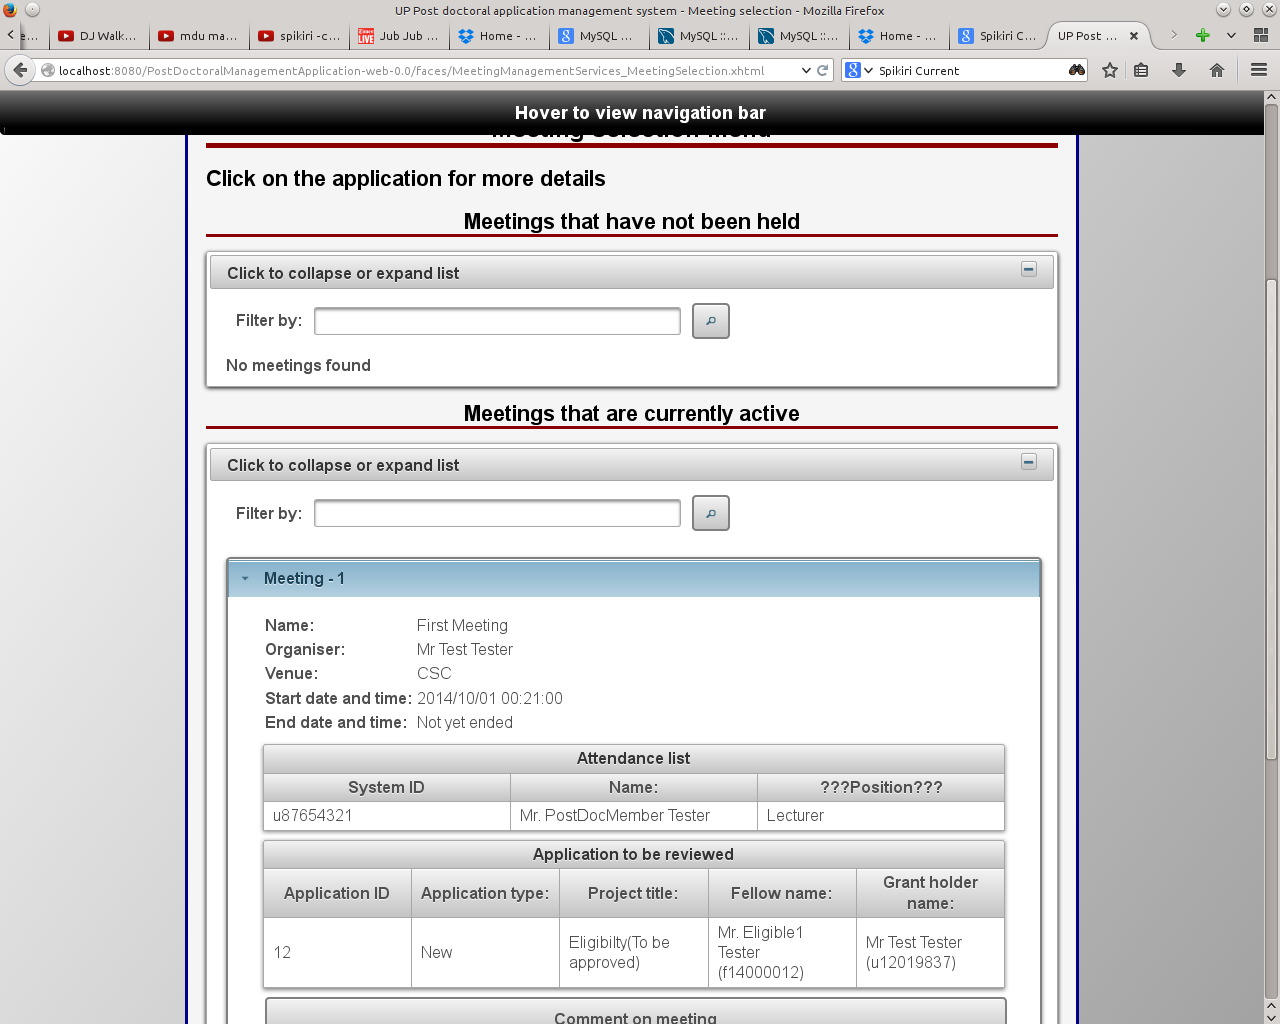
\includegraphics[scale=0.5]{../Images_Docs/Screenshots/MeetingManagementView.png}}
\caption{View Meetings}
\end{figure}

\newpage
\section{Notification}

The user will use the filters to find the notifications they require.
\begin{figure}[H]
\centering	
\framebox{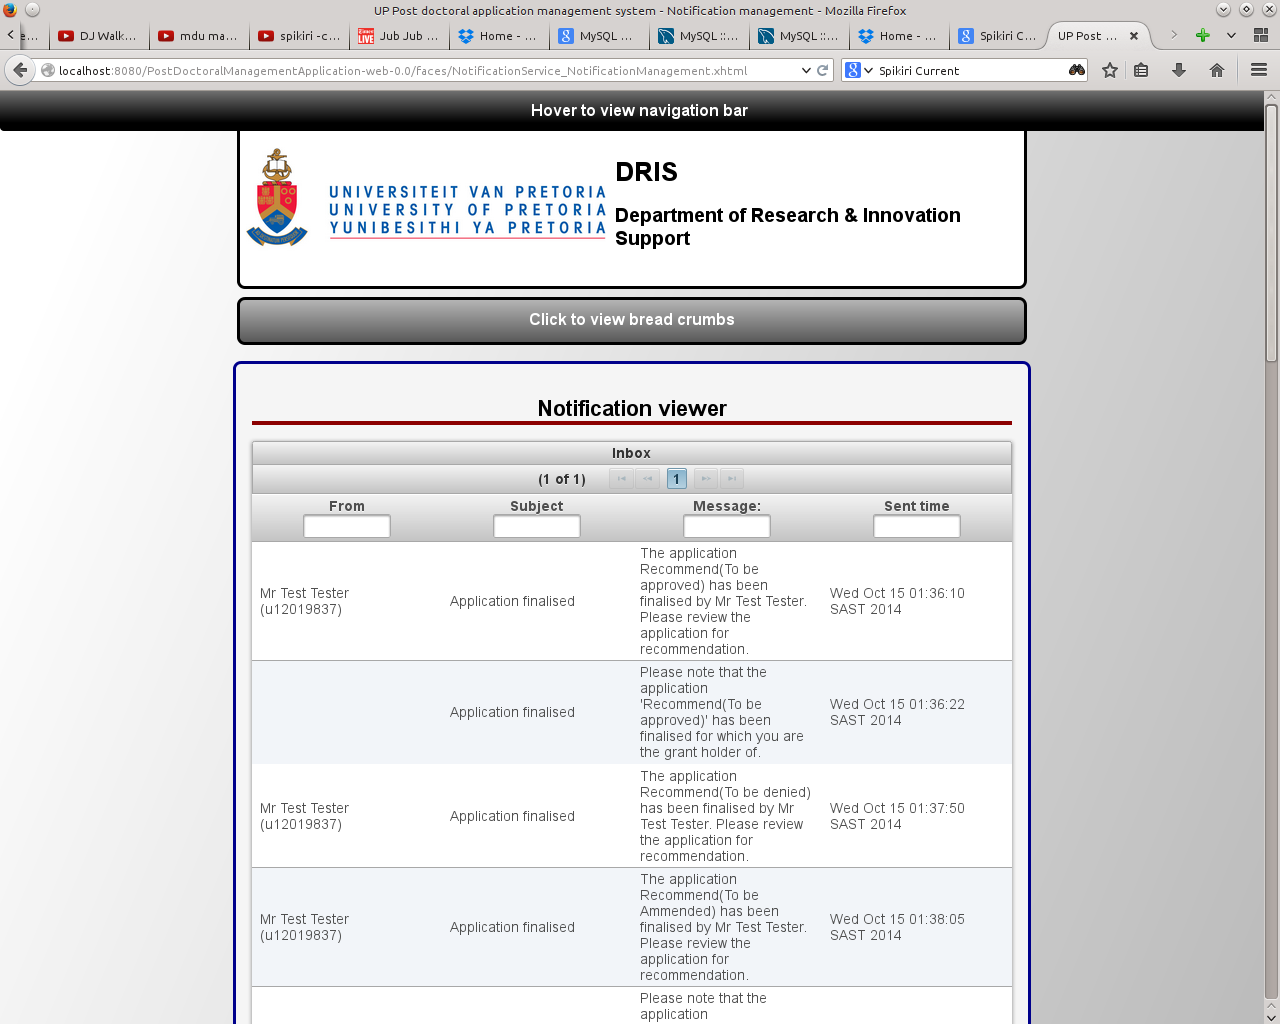
\includegraphics[scale=0.5]{../Images_Docs/Screenshots/Notification.png}}
\caption{View Notifications}

\end{figure}
\newpage
\section{Reporting Service}
The process of generating is this:
\begin{itemize}
\item Click on the Report wizard and select a query type
\begin{figure}[H]
\centering	
\framebox{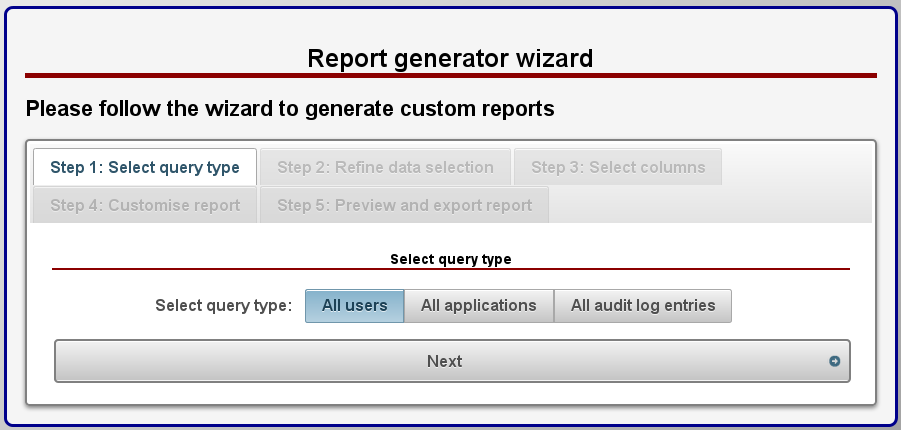
\includegraphics[scale=0.5]{../Images_Docs/Screenshots/ReportUser.png}}
\caption{View Notifications}
\end{figure}

\item Refine the selection as they see fit
\begin{figure}[H]
\centering	
\framebox{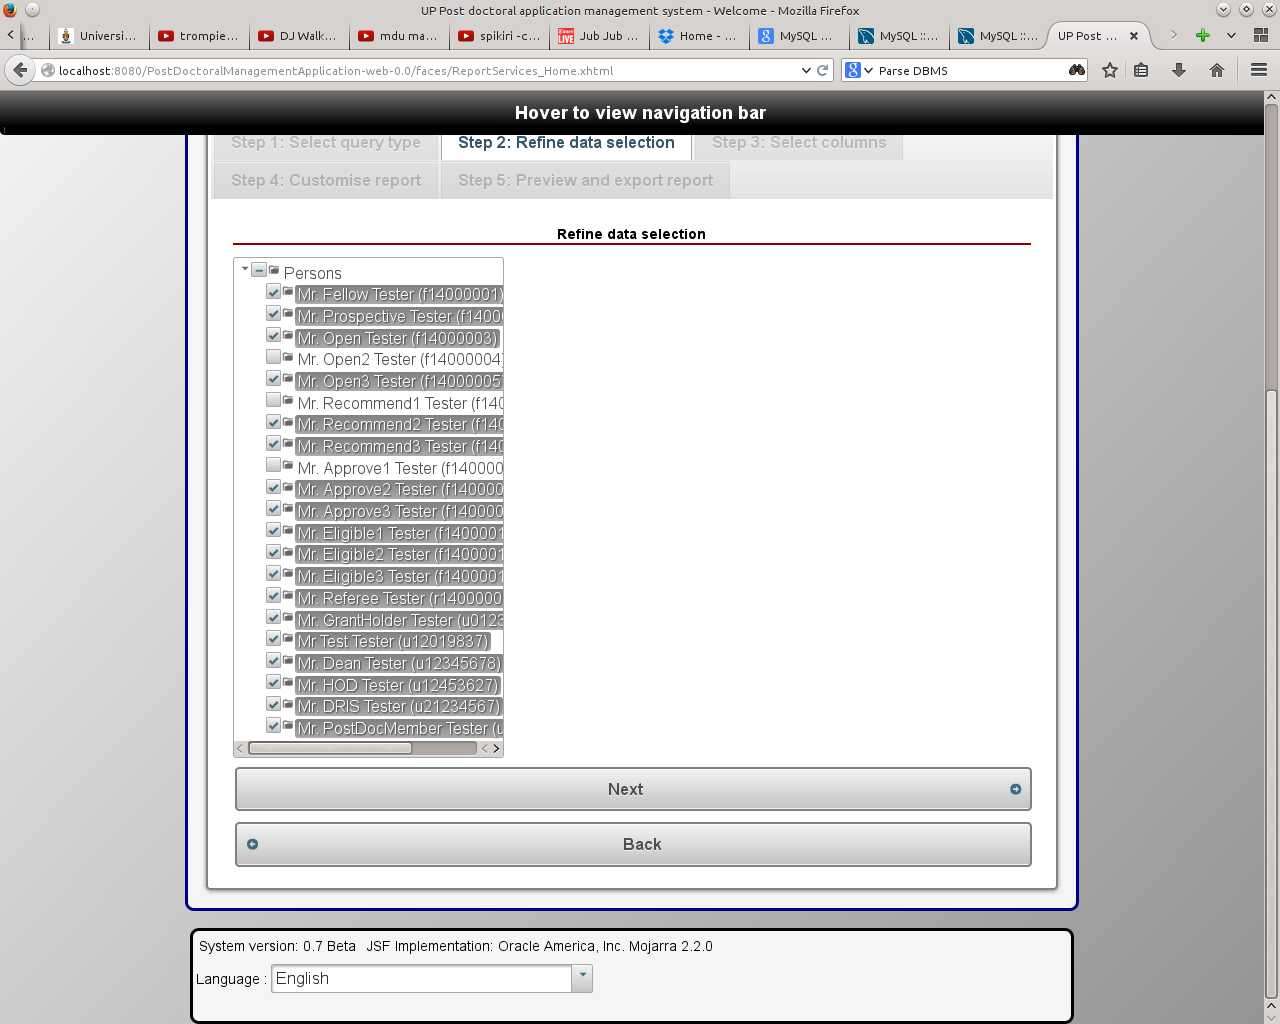
\includegraphics[scale=0.5]{../Images_Docs/Screenshots/ReportUser4.png}}
\caption{View Notifications}
\end{figure}

\item Select the columns they want to be displayed in the report.
\begin{figure}[H]
\centering	
\framebox{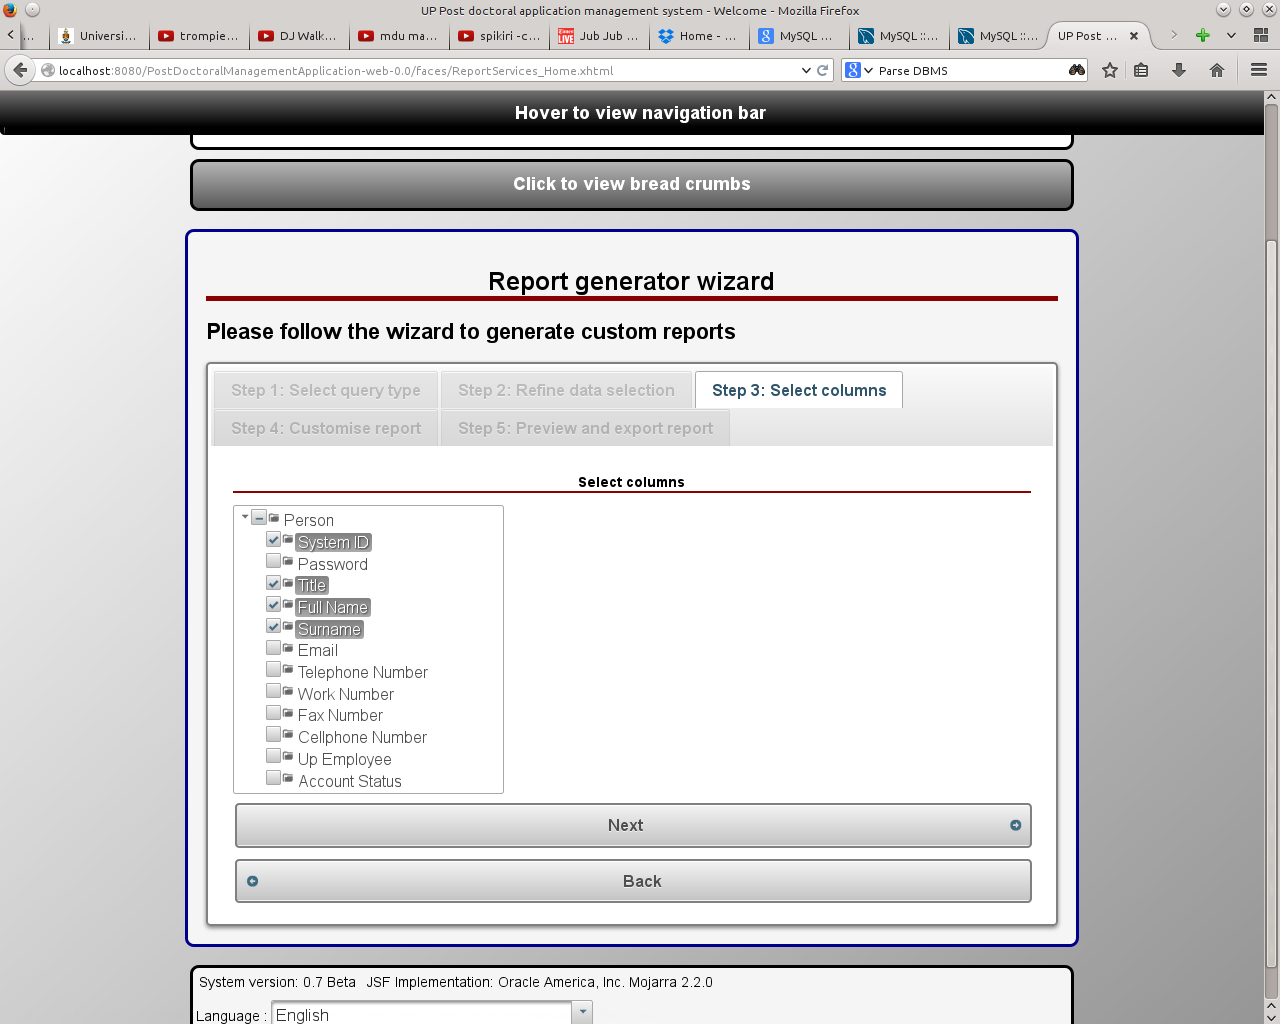
\includegraphics[scale=0.5]{../Images_Docs/Screenshots/ReportUser7.png}}
\caption{View Notifications}
\end{figure}


\item Customize the report by adding the header and name.
\begin{figure}[H]
\centering	
\framebox{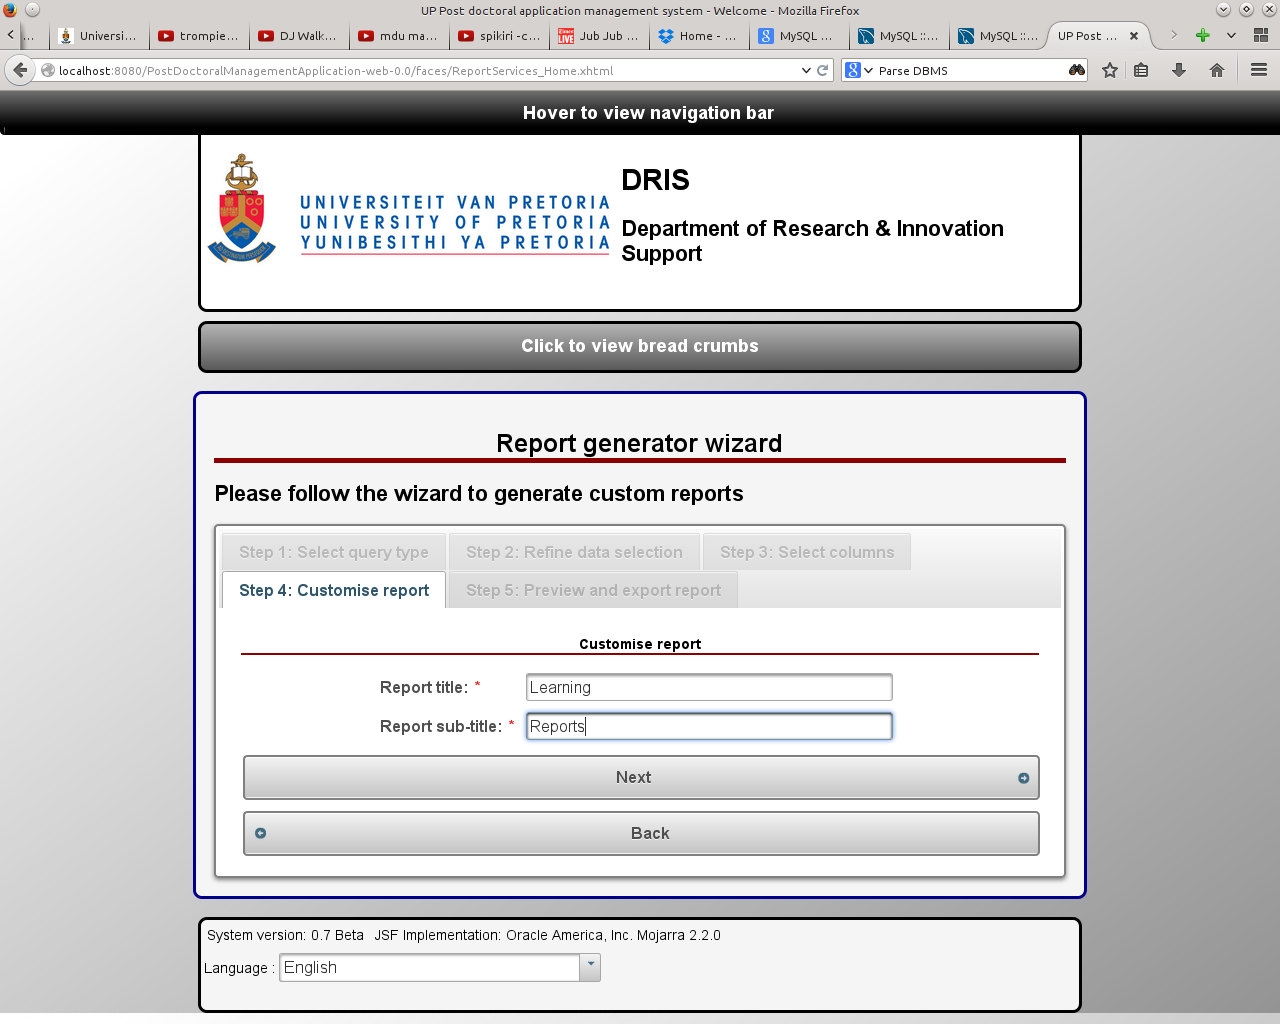
\includegraphics[scale=0.5]{../Images_Docs/Screenshots/ReportUser8.png}}
\caption{View Notifications}
\end{figure}

\item See the preview of the report and export it into the required format

\begin{figure}[H]
\centering	
\framebox{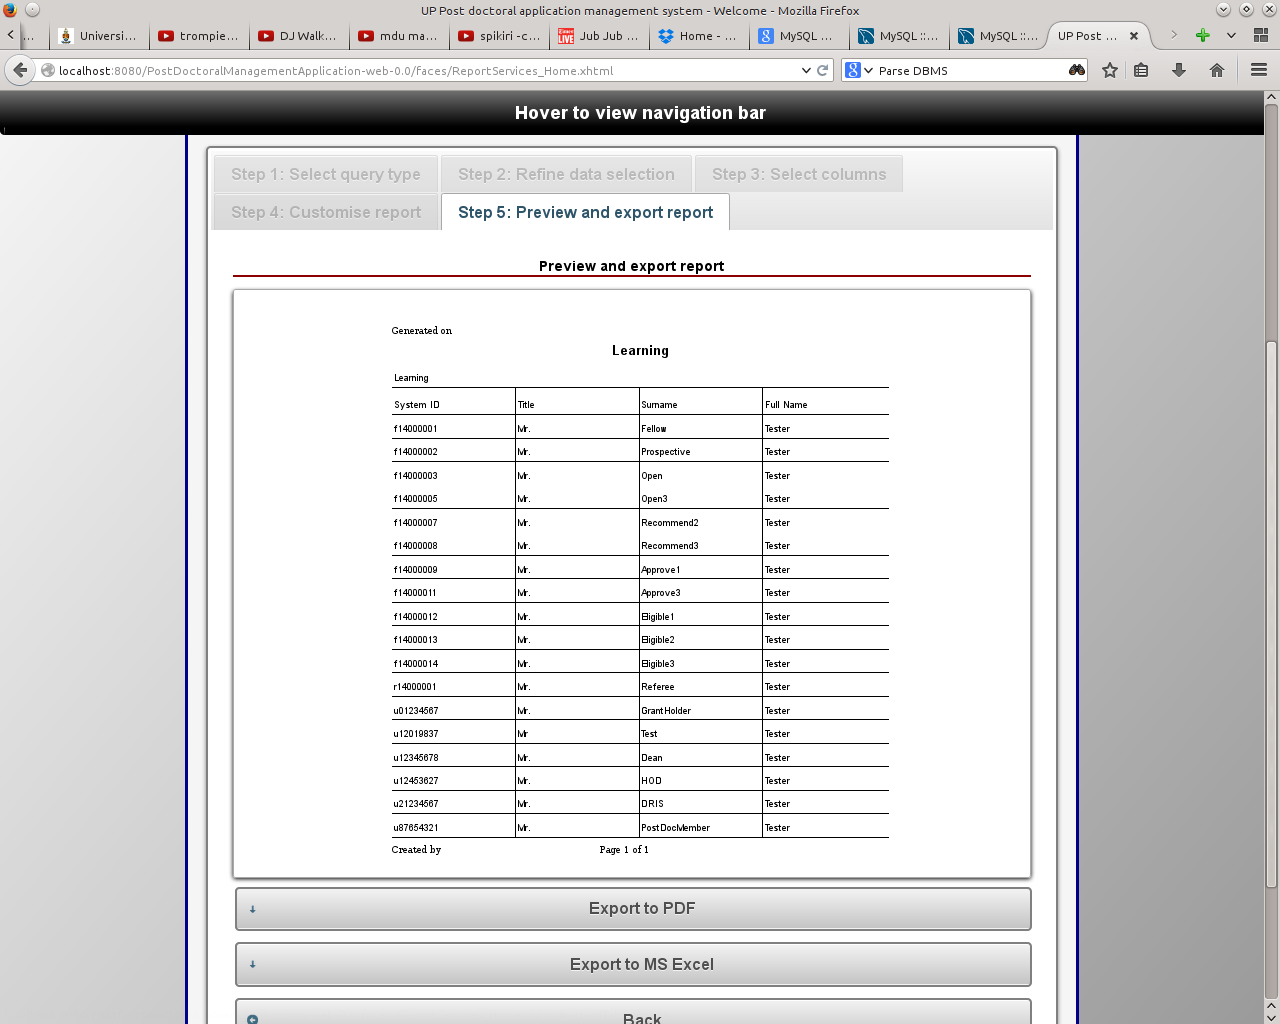
\includegraphics[scale=0.5]{../Images_Docs/Screenshots/ReportUser10.png}}
\caption{View Notifications}
\end{figure}

\item Save the report in the preferred location


\begin{figure}[H]
\centering	
\framebox{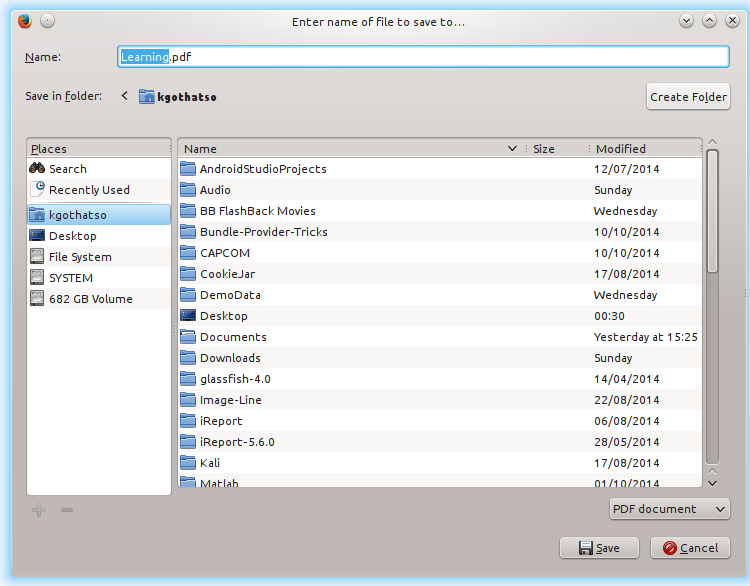
\includegraphics[scale=0.5]{../Images_Docs/Screenshots/ReportUser11.png}}
\caption{View Notifications}
\end{figure}

\end{itemize}

\newpage
\section{User Account Management}

The user will be able to edit their user information.
\begin{figure}[H]
\centering	
\framebox{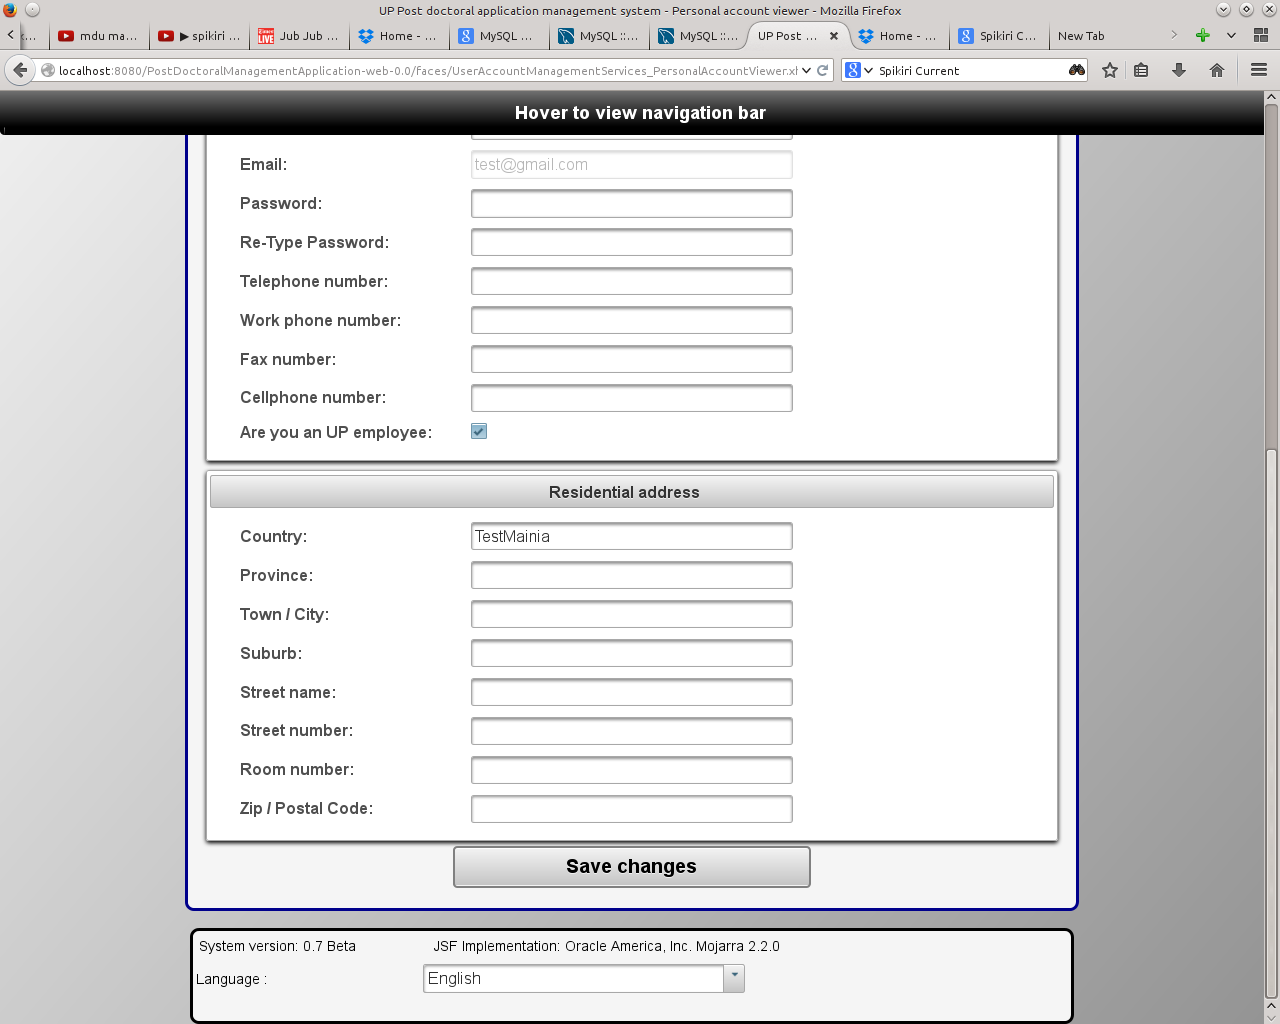
\includegraphics[scale=0.5]{../Images_Docs/Screenshots/UserAccount1.png}}
\caption{Edit User Account}

\end{figure}

The system administrator will be able to edit user accounts, by selecting an account and doing the appropriate action.
\begin{figure}[H]
\centering	
\framebox{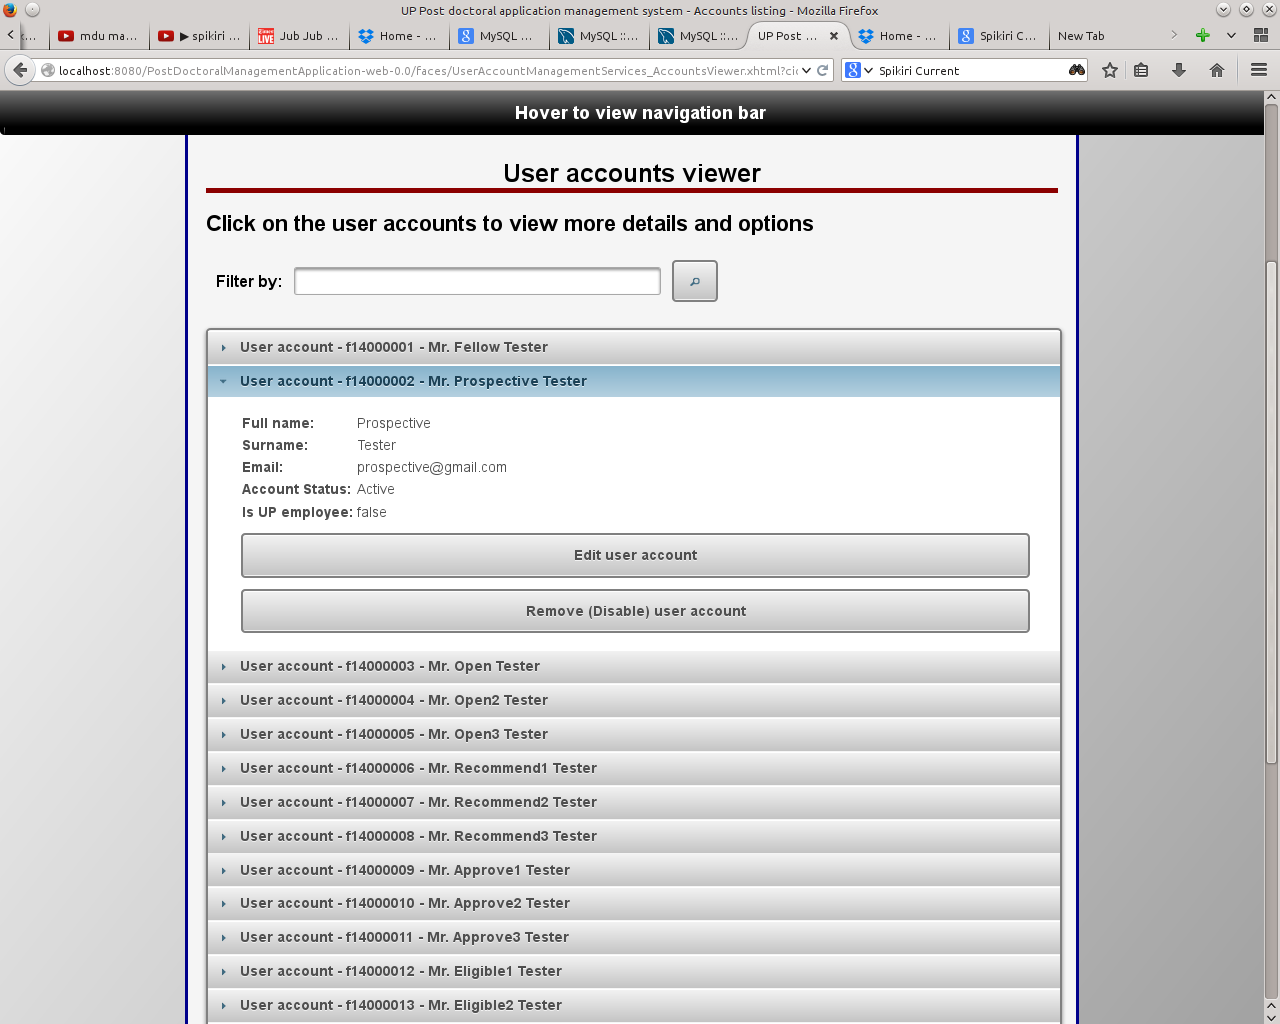
\includegraphics[scale=0.5]{../Images_Docs/Screenshots/View All Accounts1.png}}
\caption{Edit other User Accounts}

\end{figure}

\begin{figure}[H]
\centering	
\framebox{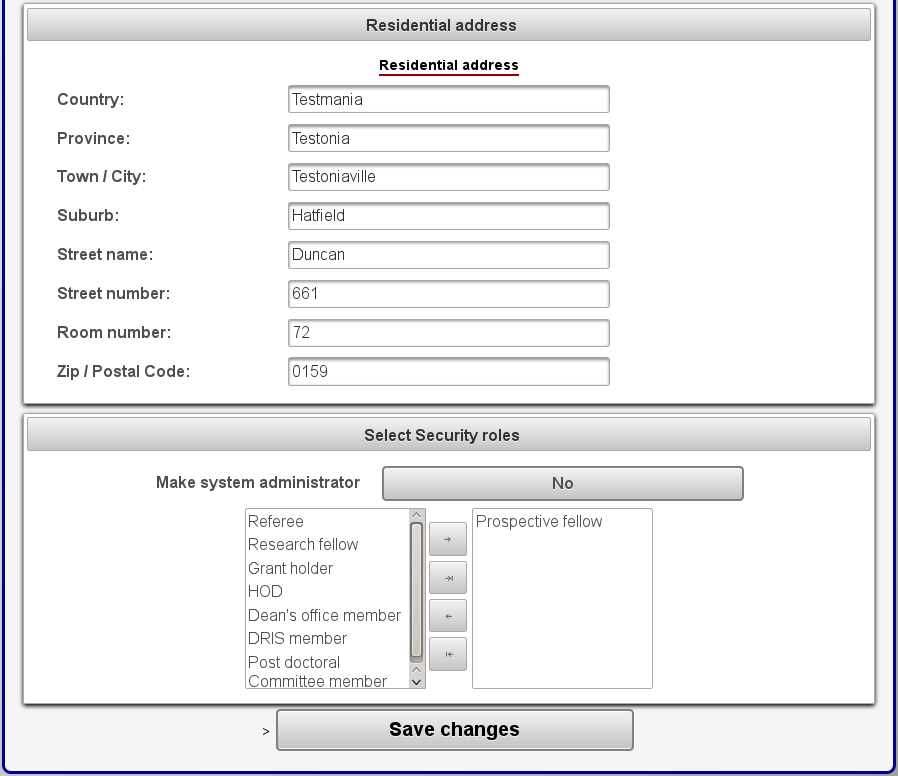
\includegraphics[scale=0.5]{../Images_Docs/Screenshots/Edit User3.png}}
\caption{Editting}
\end{figure}

\end{document}